\documentclass[remotesensing,article,submit,moreauthors,pdftex,10pt,a4paper]{Definitions/mdpi} 

\usepackage{amsmath,bm,bbm} 
\usepackage{amsfonts} 
\usepackage{subcaption}

% If you would like to post an early version of this manuscript as a preprint, you may use preprint as the journal and change 'submit' to 'accept'. The document class line would be, e.g., \documentclass[preprints,article,accept,moreauthors,pdftex,10pt,a4paper]{mdpi}. This is especially recommended for submission to arXiv, where line numbers should be removed before posting. For preprints.org, the editorial staff will make this change immediately prior to posting.

%---------
% article
%---------
% The default type of manuscript is article, but can be replaced by: 
% abstract, addendum, article, benchmark, book, bookreview, briefreport, casereport, changes, comment, commentary, communication, conceptpaper, correction, conferenceproceedings, conferencereport, expressionofconcern, extendedabstract, meetingreport, creative, datadescriptor, discussion, editorial, essay, erratum, hypothesis, interestingimages, letter, meetingreport, newbookreceived, opinion, obituary, projectreport, reply, reprint, retraction, review, perspective, protocol, shortnote, supfile, technicalnote, viewpoint
% supfile = supplementary materials
% protocol: If you are preparing a "Protocol" paper, please refer to http://www.mdpi.com/journal/mps/instructions for details on its expected structure and content.
%----------
% submit
%----------
% The class option "submit" will be changed to "accept" by the Editorial Office when the paper is accepted. This will only make changes to the frontpage (e.g., the logo of the journal will get visible), the headings, and the copyright information. Also, line numbering will be removed. Journal info and pagination for accepted papers will also be assigned by the Editorial Office.
%------------------
% moreauthors
%------------------
% If there is only one author the class option oneauthor should be used. Otherwise use the class option moreauthors.
%---------
% pdftex
%---------
% The option pdftex is for use with pdfLaTeX. If eps figures are used, remove the option pdftex and use LaTeX and dvi2pdf.

%=================================================================
\firstpage{1} 
\makeatletter 
\setcounter{page}{\@firstpage} 
\makeatother
\pubvolume{xx}
\issuenum{1}
\articlenumber{5}
\pubyear{2019}
\copyrightyear{2019}
%\externaleditor{Academic Editor: name}
\history{Received: date; Accepted: date; Published: date}
%\updates{yes} % If there is an update available, un-comment this line

%% MDPI internal command: uncomment if new journal that already uses continuous page numbers 
%\continuouspages{yes}

%------------------------------------------------------------------
% The following line should be uncommented if the LaTeX file is uploaded to arXiv.org
%\pdfoutput=1

%=================================================================
% Add packages and commands here. The following packages are loaded in our class file: fontenc, calc, indentfirst, fancyhdr, graphicx, lastpage, ifthen, lineno, float, amsmath, setspace, enumitem, mathpazo, booktabs, titlesec, etoolbox, amsthm, hyphenat, natbib, hyperref, footmisc, geometry, caption, url, mdframed, tabto, soul, multirow, microtype, tikz

%=================================================================
%% Please use the following mathematics environments: Theorem, Lemma, Corollary, Proposition, Characterization, Property, Problem, Example, ExamplesandDefinitions, Hypothesis, Remark, Definition
%% For proofs, please use the proof environment (the amsthm package is loaded by the MDPI class).

%=================================================================
% Full title of the paper (Capitalized)
\Title{Texture Analysis with Information Theory}

% Author Orchid ID: enter ID or remove command
\newcommand{\orcidauthorA}{0000-0000-000-000X} % Add \orcidA{} behind the author's name
%\newcommand{\orcidauthorB}{0000-0000-000-000X} % Add \orcidB{} behind the author's name

% Authors, for the paper (add full first names)
\Author{Eduarda C.\ Chagas $^{1,\dagger,\ddagger}$\orcidA{}, 
	Roger de A.\ Matos Júnior $^{2,\ddagger}$, 
	Heitor S.\ Ramos$^{1}$, Osvaldo A.\ Rosso $^{2,}$* and
	Alejandro C.\ Frery$^{2,\ddagger}$\orcidA{}}
%%% ORCID Alejandro 0000000280025341

% Authors, for metadata in PDF
\AuthorNames{Firstname Lastname, Firstname Lastname and Firstname Lastname}

% Affiliations / Addresses (Add [1] after \address if there is only one affiliation.)
\address{%
	$^{1}$ \quad Department of Computer Science, Federal University of Minas Gerais, Belo Horizonte, Brazil; eduarda-chagas@ufmg.com.br\\
	$^{2}$ \quad Laboratório de Computação Científica e Análise Numérica, Universidade Federal de Alagoas, Maceió, Brazil; acfrery@laccan.ufal.br}

% Contact information of the corresponding author
%\corres{Correspondence: e-mail@e-mail.com; Tel.: +x-xxx-xxx-xxxx}

% Current address and/or shared authorship
%\firstnote{Current address: Affiliation 3} 
%\secondnote{These authors contributed equally to this work.}
% The commands \thirdnote{} till \eighthnote{} are available for further notes

%\simplesumm{} % Simple summary

%\conference{} % An extended version of a conference paper

\abstract{}

% Keywords
\keyword{Texture images, Spatial patterns; Permutation Entropy; Complexity; Ordinal patterns probabilities}

% The fields PACS, MSC, and JEL may be left empty or commented out if not applicable
%\PACS{J0101}
%\MSC{}
%\JEL{}

%%%%%%%%%%%%%%%%%%%%%%%%%%%%%%%%%%%%%%%%%%
% Only for the journal Diversity
%\LSID{\url{http://}}

%%%%%%%%%%%%%%%%%%%%%%%%%%%%%%%%%%%%%%%%%%
% Only for the journal Applied Sciences:
%\featuredapplication{Authors are encouraged to provide a concise description of the specific application or a potential application of the work. This section is not mandatory.}
%%%%%%%%%%%%%%%%%%%%%%%%%%%%%%%%%%%%%%%%%%

%%%%%%%%%%%%%%%%%%%%%%%%%%%%%%%%%%%%%%%%%%
% Only for the journal Data:
%\dataset{DOI number or link to the deposited data set in cases where the data set is published or set to be published separately. If the data set is submitted and will be published as a supplement to this paper in the journal Data, this field will be filled by the editors of the journal. In this case, please make sure to submit the data set as a supplement when entering your manuscript into our manuscript editorial system.}

%\datasetlicense{license under which the data set is made available (CC0, CC-BY, CC-BY-SA, CC-BY-NC, etc.)}

%%%%%%%%%%%%%%%%%%%%%%%%%%%%%%%%%%%%%%%%%%
% Only for the journal Toxins
%\keycontribution{The breakthroughs or highlights of the manuscript. Authors can write one or two sentences to describe the most important part of the paper.}

%\setcounter{secnumdepth}{4}
%%%%%%%%%%%%%%%%%%%%%%%%%%%%%%%%%%%%%%%%%%
\begin{document}
	%%%%%%%%%%%%%%%%%%%%%%%%%%%%%%%%%%%%%%%%%%
	%% Only for the journal Gels: Please place the Experimental Section after the Conclusions
	
	%%%%%%%%%%%%%%%%%%%%%%%%%%%%%%%%%%%%%%%%%%
	%\setcounter{section}{-1} %% Remove this when starting to work on the template.
	
	%The order of the section titles is: Introduction, Materials and Methods, Results, Discussion, Conclusions
	
	\section{Introdução}
	
	A análise de texturas possui um grande poder informacional das propriedades espaciais dos principais elementos da imagem, sendo uma das técnicas mais importantes no processamento de imagens e reconhecimento de padrões, uma vez que uma boa compreensão ou uma interpretação das imagens deve incluir a descrição dos aspectos espectrais e texturais da mesma. 
	A informação textural às vezes pode ser a única maneira de caracterizar uma imagem digital.
	
	A primeira tarefa na análise de texturas consiste na extração de características discriminantes, capazes de incorporar de modo eficiente informações sobre as características da imagem original.
	Esses recursos podem ser usados para a descrição ou classificação de diferentes texturas usando qualquer uma das várias técnicas de reconhecimento de padrões~\cite{Lee1994Texture}.
	
	Neste trabalho propomos uma nova metodologia de caracterização de texturas. 
	Ao receber uma textura realizamos o processo de linearização aplicando \textit{space filling curves} e por meio da simbolização de Bandt \& Pompe~\cite{Bandt2002Permutation} usamos o poder discriminatório da Teoria da Informação para realizar a caracterização.
	Duas análises foram usadas para validar a abordagem proposta.
	Na primeira, avaliamos como podemos utilizar descritores causais da Teoria da Informação na caracterização de texturas de Brodatz. 
	Na segunda, usamos o plano Entropia-Complexidade em diferentes regiões extraídas de texturas provenientes de imagens \texttt{SAR}.
	
	O artigo foi dividido do seguinte modo: Na seção~\ref{Curves}, as \textit{spaces filling curves} são apresentadas; na seção~\ref{HC}, introduzimos a simbolização de Bandt \& Pompe e os descritores da Teoria da Informação; na seção~\ref{Metodologia}, nossa metodologia é proposta; na seção~\ref{Resultados}, mostramos os resultados obtidos nas duas análises aplicadas; e por último na seção~\ref{conclusao}, concluímos o trabalho e citamos os trabalhos futuros considerados. 
	
	%%%%%%%%%%%%%%%%%%%%%%%%%%%%%%%%%%%%%%%%%%
	\section{Space Filling Curves}\label{Curves}
	
	As \textit{space filling curves} foram vistas pela primeira vez em~\cite{Nguyen1982SpaceFC}, transformando uma imagem de textura em um sinal unidimensional. Diferentes comprimentos destes sinais foram então calculados em diferentes faixas de suavização e usados como um parâmetro de característica para a análise de textura.
	
	Quando usadas como métodos de varredura de uma imagem, tais funções conseguem preservar bem as propriedades eminentes da correlação espacial dos pixels, embora não forneçam um poder discriminatório suficiente para classificar texturas naturais~\cite{Lee1994Texture}. Neste artigo, objetivamos verificar o poder de caracterização de texturas das curvas \texttt{raster-1}, \texttt{raster-2} e \texttt{Hilbert} (exibidas na figura~\ref{fig:FillingCurves}), quando usadas em conjunto com a simbolização de~\cite{Bandt2002Permutation} e os descritores da Teoria da Informação. 
	
	Assumindo que uma imagem é uma grade $N \times N$ de pixels, onde $N$ é uma potência de $2$, temos: 
	
	\newtheorem{mydef}{Definição}
	\begin{mydef}
		Uma varredura da imagem é uma função bijetora $f: \mathbb{N} \times \mathbb{N} \to \mathbb{N}$ no conjunto de pares ordenados $\{(i,j) | 1\leq i,j \leq N\}$, que denota os pontos no domínio, para o intervalo fechado de inteiros $\{1, \dots, N^2\}$. Equivalentemente, a imagem é codificada usando a varredura $f$ nas intensidades de pixel na ordem $P_{f^{-1}(1)}, P_{f^{-1}(2)}, \dots, P_{f^{-1}(N^2)}$, onde $P_{(i,j)}$ representa a intensidade do pixel da coluna $i$ e linha $j$.
		\label{def:CurveFilling}
	\end{mydef}
	
	As \textit{space filling curves}, como as técnicas de varredura \texttt{raster-1}, \texttt{raster-2} e \texttt{Hilbert} são caracterizadas pela definição~\ref{def:CurveFilling}, fornecendo uma função adequada $f$. Como também pode ser observado pela definição~\ref{def:CurveFilling}, as curvas nos impõe a condição de que cada pixel seja visitado apenas uma vez.
	
	\begin{figure}[hbt]
		\centering
		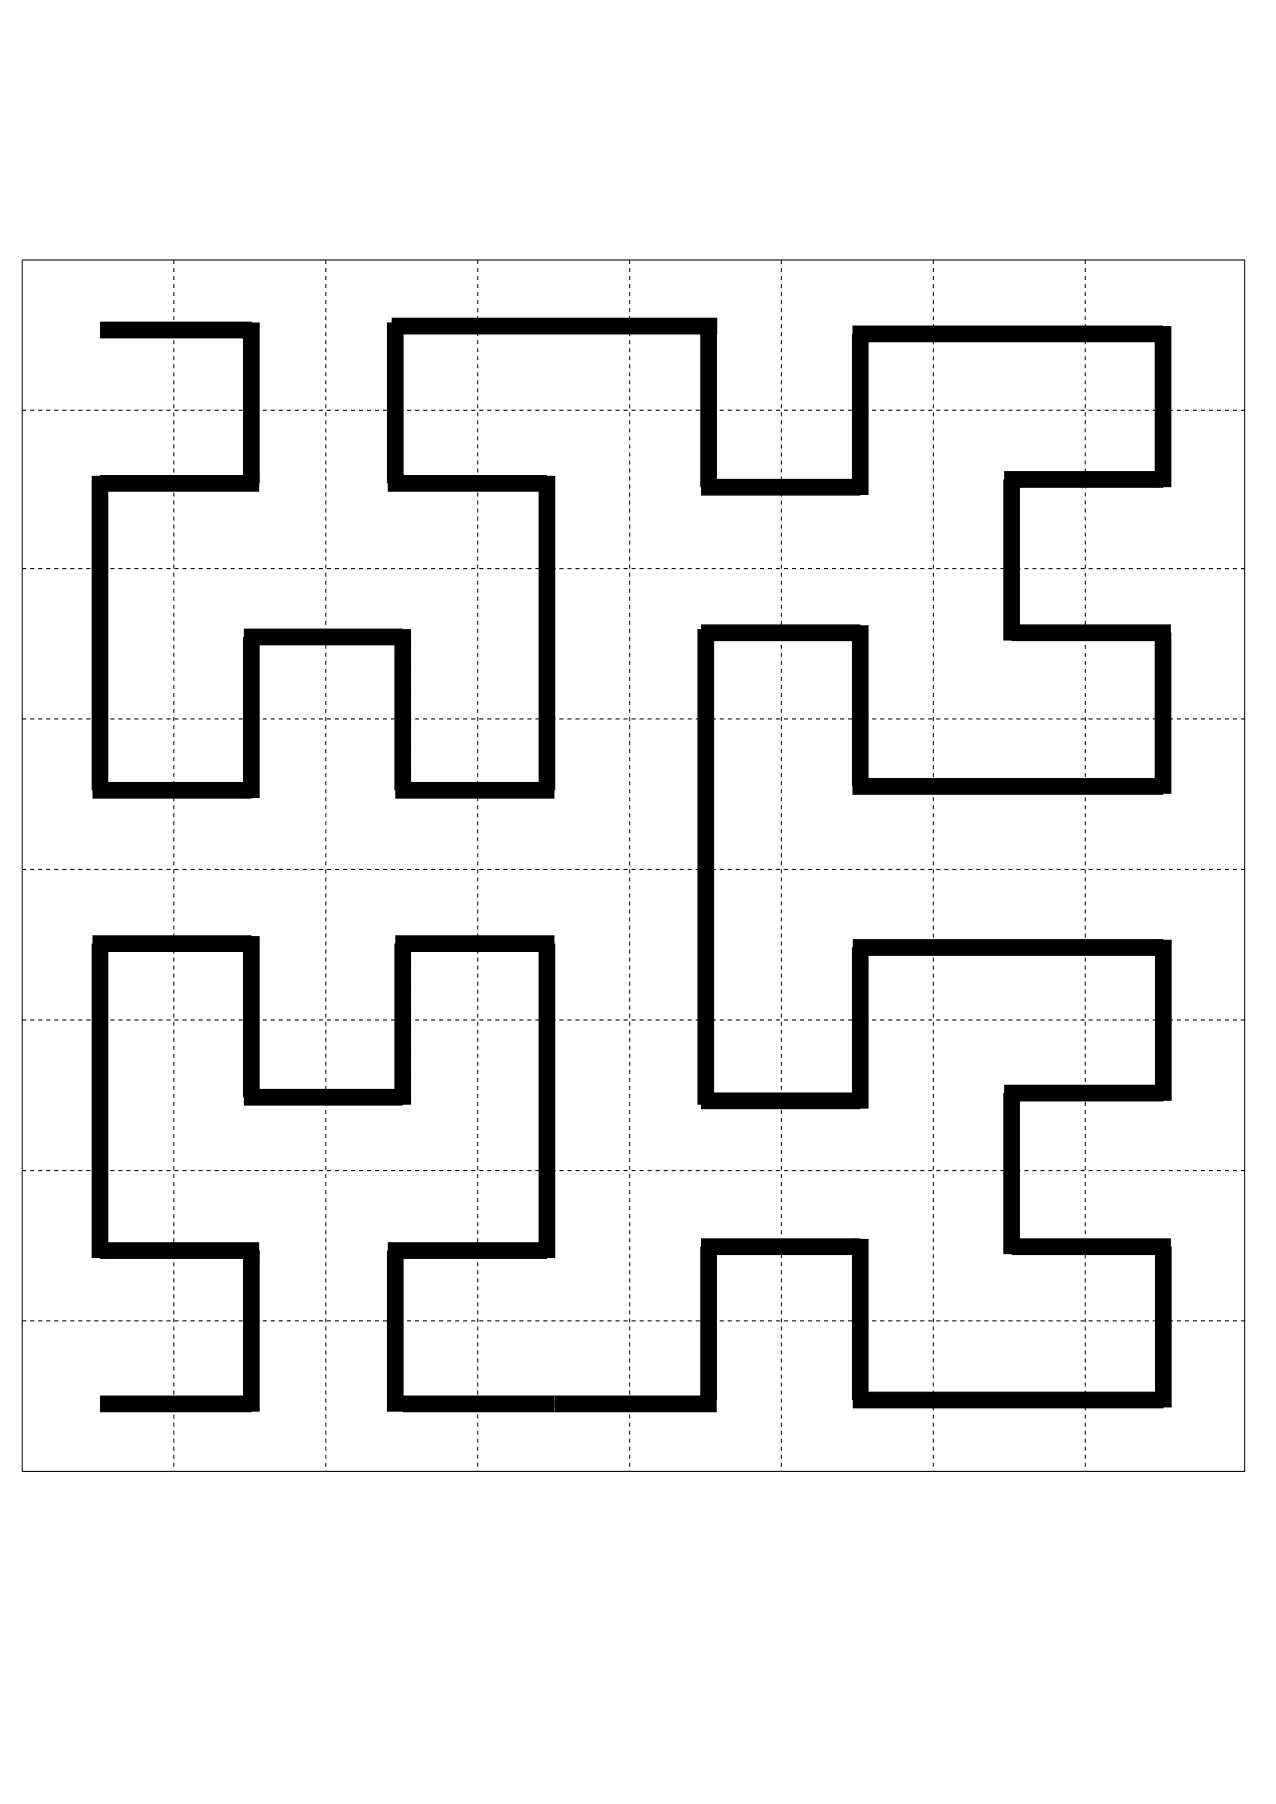
\includegraphics[width=2.5cm,height=3.5cm]{Figures/hilbert.png}
		
\includegraphics[width=2.5cm,height=3.5cm]{Figures/raster1.png}
		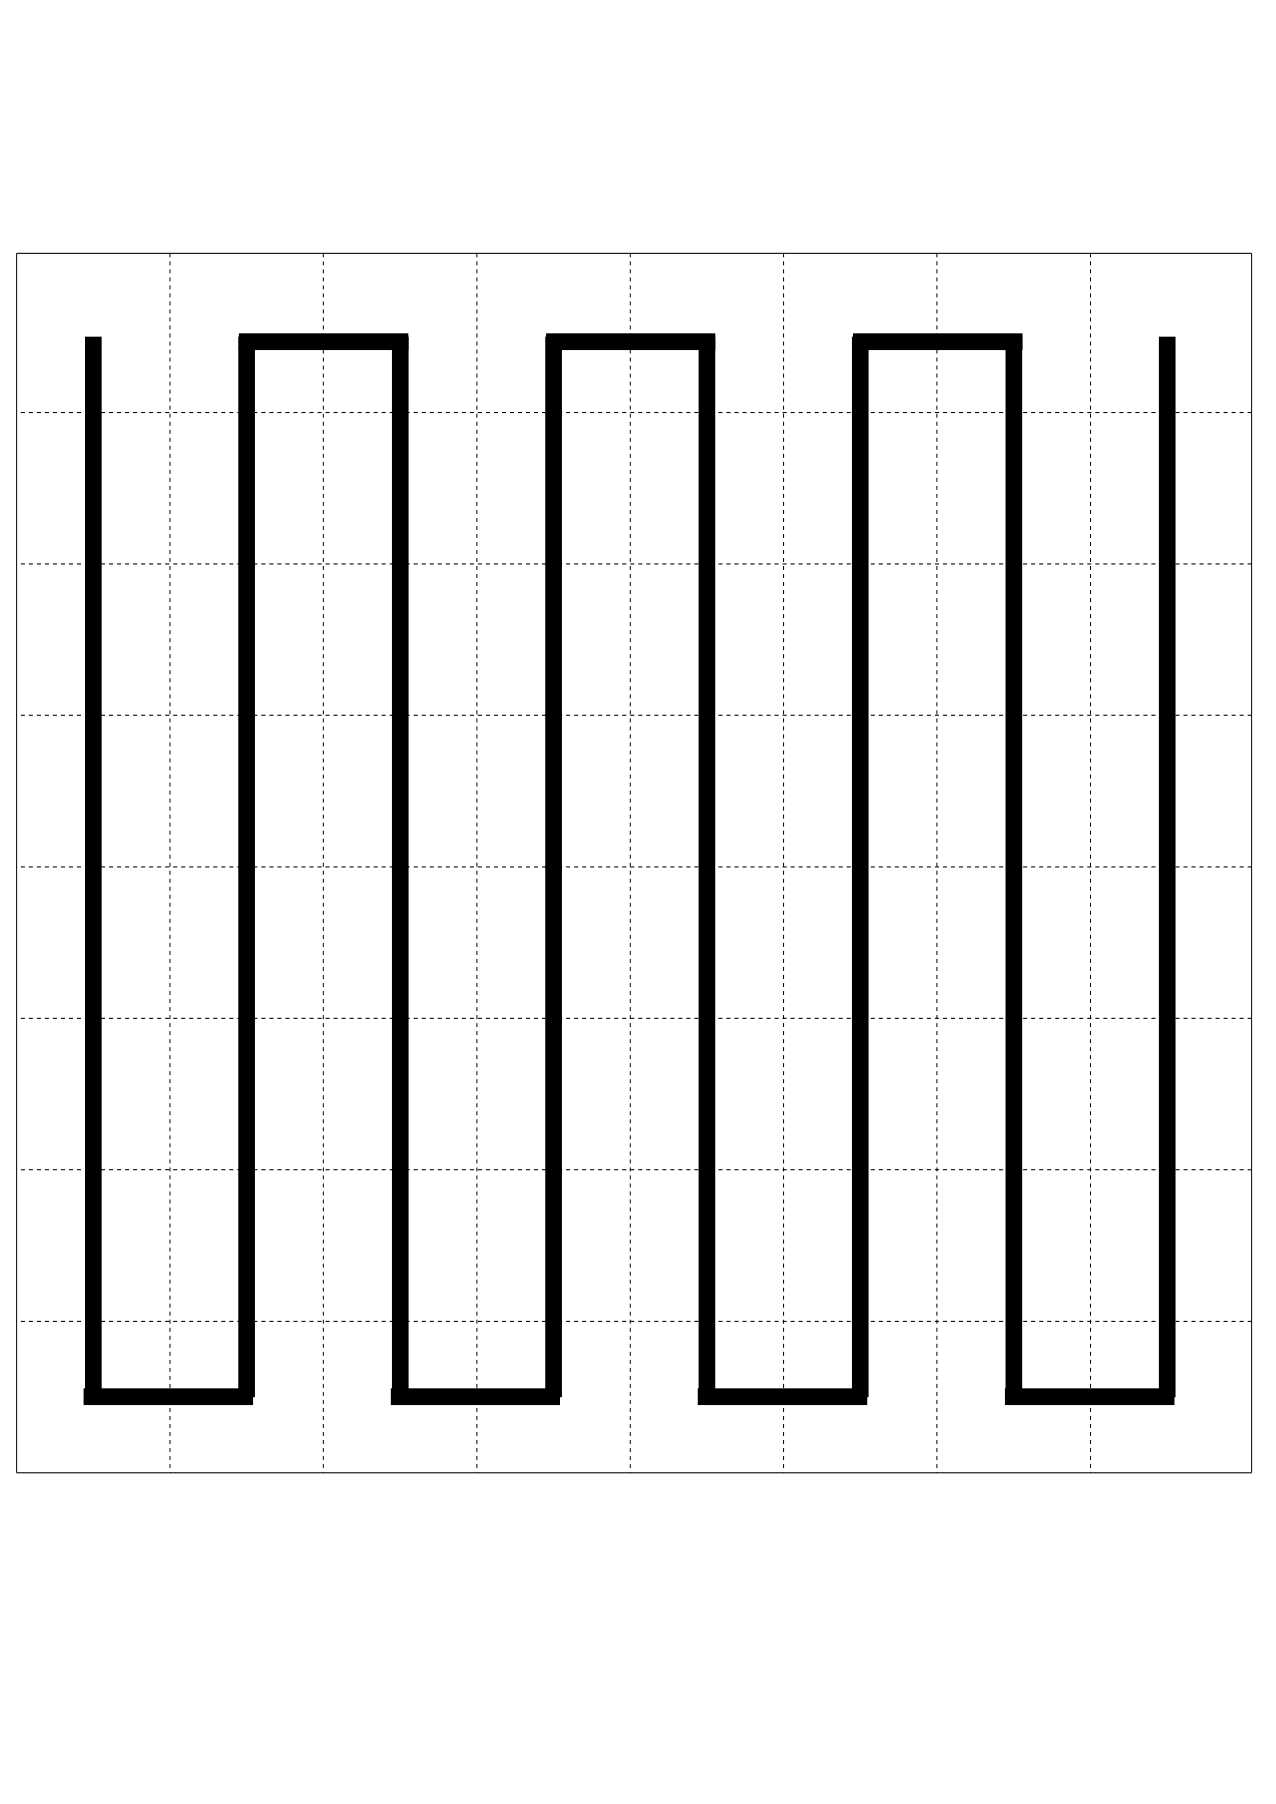
\includegraphics[width=2.5cm,height=3.5cm]{Figures/raster2.png}
		\vspace{-0.5cm}
		\caption{A janela 8x8 das \textit{space filling curves} usadas: (a) \texttt{Hilbert}; (b) \texttt{Raster-1}; (c) \texttt{Raster-2}.}
		\label{fig:FillingCurves}
	\end{figure}
	
	Para as curvas de rasterização, algumas modificações foram realizadas para facilitar o processo de simbolização de bandt \& Pompe descrito na seção seguinte. 
	
	O primeiro passo foi definir as submatrizes deslizantes e para isso quatro parâmetros foram necessários: As dimensões $D_{x}, D_{y} \geq 2$, que são o número de elementos que formam os padrões ordinais em ambas dimensões e os delays $\tau _{x}$ e $\tau_{y}$, que informam o quão separados espacialmente estão os símbolos nas duas direções. Após realizar esta subdivisão, devemos investigar quais padrões aparecem dentro dos elementos das submatrizes analisando os elementos destes conjuntos linha por linha.
	
	%%%%%%%%%%%%%%%%%%%%%%%%%%%%%%%%%%%%%%%%%%
	\section{Plano Entropia-Complexidade}\label{HC}
	
	A transformação de uma série temporal em uma distribuição de probabilidade (\texttt{PDF}) \texttt{P} permite avaliar o conteúdo informacional acerca da dinâmica do sistema e dos processos subjacentes, descrevendo-os de forma mensurável e observável~\cite{Gray1990Entropy}.
	Através desta caracterização é possível utilizar de métricas do espaço \texttt{PDF}, permitindo comparar diferentes conjuntos e classificá-los de acordo com as propriedades dos processos subjacentes. 
	
	No entanto, não é trivial encontrar uma representação simbólica significativa da série original. 
	A abordagem de Bandt \& Pompe~\cite{Bandt2002Permutation}, por considerar a causalidade temporal dos dados, revela detalhes importantes da estrutura ordinal da série temporal.
	
	A metodologia de Bandt \& Pompe consiste na transformação não paramétrica da série temporal em uma sequência de padrões. 
	Seja a série temporal $\bm x = (x_1, x_2, \dots, x_N)$, cada grupo de $D$ valores (não necessariamente adjacentes) será transformado em um padrão ordinal, para depois formar o histograma das suas ocorrências na série.
	Por exemplo, com $D=3$ e para qualquer $0 \leq i \leq D$,
	se $x_i<x_{i+1}<x_{i+2}$ esta tripla será associada ao padrão $\pi_0$; 
	caso $x_i>x_{i+1}>x_{i+2}$ o padrão será $\pi_1$, e assim por diante.
	Há $D!$ possíveis padrões.
	
	Esta simbolização é muito resistente a vários tipos de contaminação, por exemplo, o padrão $\pi_0$ não será alterado para qualquer $k>1$ que afete multiplicativamente $x_{i+2}$.
	Ainda que o padrão seja alterado, por exemplo se $k=-1$, a mudança será local e afetará, no máximo, $D$ padrões.
	
	Forma-se, então, um histograma e, a partir dele, extraem-se quantificadores como, por exemplo, entropia, distância estocástica a uma distribuição de equilíbrio, e complexidade estatística.
	
	Seja, assim, $\bm h=(h_1,\dots,h_{D!})$ o histograma de probabilidade dos $D!$ padrões observados a partir da série temporal $\bm X$.
	Calculamos a entropia de Shannon
	\begin{equation}
	H(\bm h) = \sum_{i=1}^{D!} (-\log h_i) h_i,
	\label{eq:Entropia}
	\end{equation}
	
	A entropia de Shannon é o primeiro elemento a descrever a nossa série temporal.
	Ela mede a desordem do sistema que deu origem aos dados $\bm X$.
	
	Calculamos a distância de Jensen-Shannoon à distribuição uniforme $\bm u=(1/D!,\dots,1/D!)$
	\begin{equation}
	D(\bm h,\bm u) = \sum_{i=1}^{D!} \Big(h_i \log\frac{h_i}{u_i} +
	u_i \log\frac{u_i}{p_i}
	\Big),
	\end{equation}
	em que $u_i=1/D!$.
	Esta é uma medida de quão perto ou longe a dinâmica subjacente está de um processo sem informação nenhuma.
	
	Finalmente, calculamos a Complexidade Estatística:
	\begin{equation}
	C(\bm h, \bm u) = H(\bm h) D(\bm h, \bm u).
	\end{equation}
	
	Cada série temporal pode então ser descrita por um ponto $(H(\bm h), C(\bm h, \bm u))$.
	O conjunto de todos os pares $(H(\bm h), C(\bm h, \bm u))$ para qualquer série temporal descrita por padrões de comprimento $D$ jaz em um subconjunto compacto $\mathbbm R^2$: o plano Entropia-Complexidade.
	
	%%%%%%%%%%%%%%%%%%%%%%%%%%%%%%%%%%%%%%%%%%
	\section{Metodologia Proposta}\label{Metodologia}
	
	O algoritmo de caracterização proposto para análise de texturas naturais consiste em dois módulos, que são a linearização dos dados da matriz de intensidade da imagem e a representação dos sinais correspondentes por meio do Plano Entropia-Complexidade. A linearização foi realizada com cada uma das \textit{space filling curves} mostradas na figura~\ref{fig:FillingCurves} e analisada a influência de seus respectivos mapeamentos no plano Entropia-Complexidade.
	
	Na figura~\ref{fig:MethodologySAR}, verificamos que é usado como input uma textura proveniente de uma dada imagem \texttt{SAR}, entretanto é importante destacar que a entrada para a metodologia proposta neste trabalho não é influenciada pela semântica dos dados, recebendo, de forma genérica, qualquer matriz bidimensional com valores pertencentes ao conjunto dos números reais ($\mathbb{R}$).
	
	\begin{figure}[!h]
		\centering
		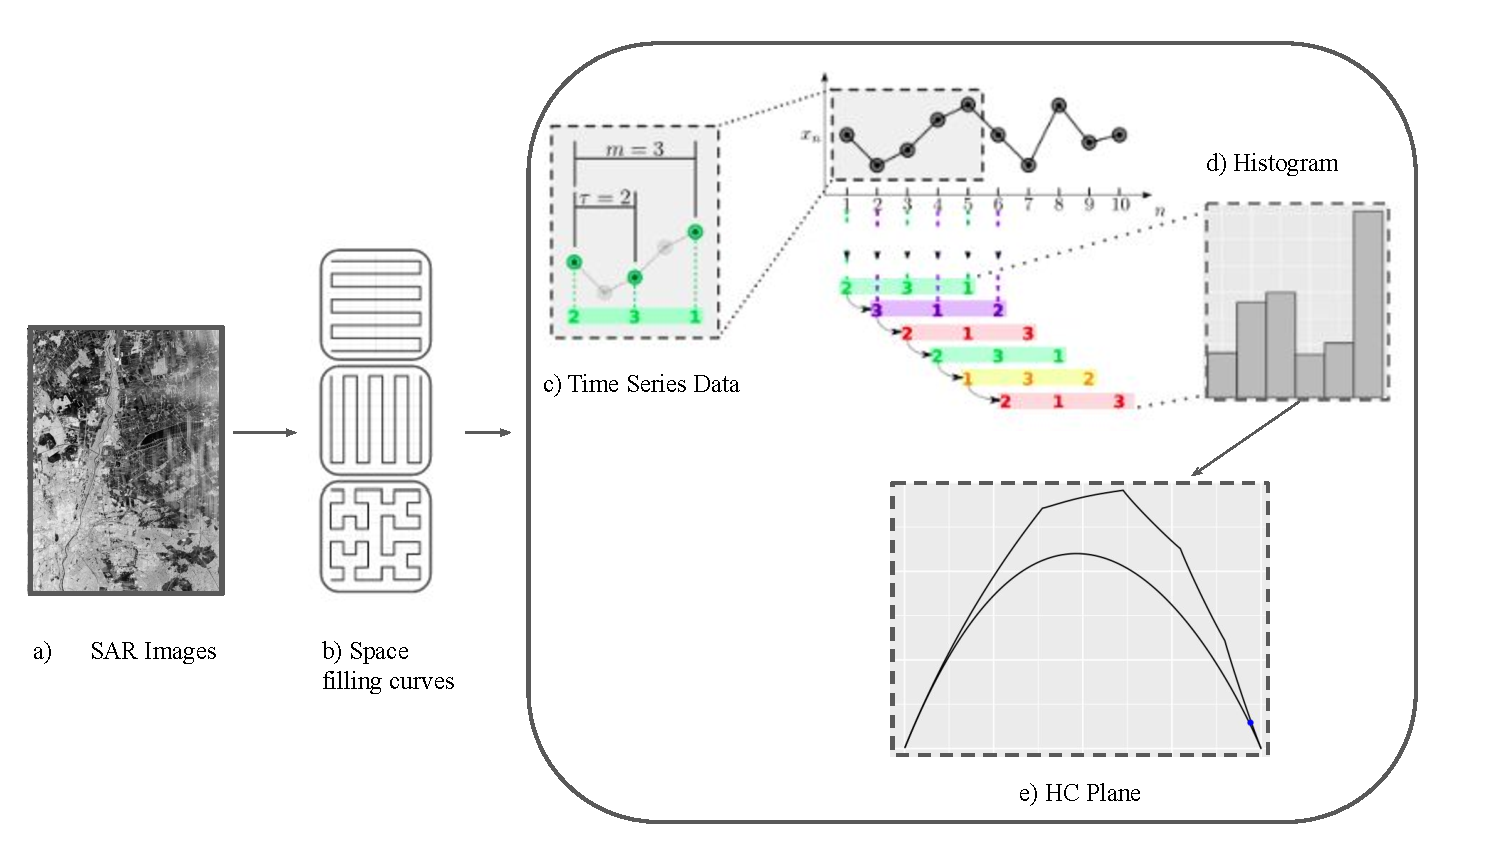
\includegraphics[scale = 0.5]{Figures/MethodologySAR.pdf}    
		\caption{Metodologia usada na caracterização das imagens \texttt{SAR}}
		\label{fig:MethodologySAR}
	\end{figure}
	
	A implementação geral da caracterização de imagens de texturas pode ser descrita de acordo com as seguintes etapas:
	
	\begin{enumerate}
		\item \textbf{Tratamento da entrada}. Devido restrições da curva de \texttt{Hilbert}, as imagens recebidas como entrada devem possuir dimensões em potência de 2, logo esta restrição deve ser primeiramente verificada.
		\item \textbf{Seleção da função de mapeamento}. Apenas um método de varredura é utilizado em cada análise. Nesta etapa realizamos a transformação de dados bidimensional para sinais unidimensionais.
		\item \textbf{Simbolização de Bandt \& Pompe}. Calculamos a distribuição de probabilidade dos dados para assim conseguirmos aplicar os quantificadores da Teoria da Informação.
		\item \textbf{Plano Entropia-Complexidade}. Representando a nossa principal ferramenta de caracterização, é nesta etapa que verificamos o comportamento da dinâmica dos dados resultantes do mapeamento e consequentemente do seu poder de discriminação.
	\end{enumerate}
	
	%%%%%%%%%%%%%%%%%%%%%%%%%%%%%%%%%%%%%%%%%%
	\section{Experimentos e Resultados}\label{Resultados}
	
	Para avaliar a metodologia proposta para caracterização e discriminação de texturas de imagens, usamos dois exemplos de aplicações. O primeiro consiste em realizar um estudo empírico do comportamento dos descritores da Teoria da Informação quando aplicamos imagens de textura natural de Brodatz. O segundo exemplo consiste em analisar amostras de imagens de quatro diferentes tipos de regiões em uma imagem de radar de abertura sintética (\texttt{SAR}) usando os valores de entropia de permutação de Shannon e Complexidade Estatística. Os dados das imagens, as características das analisadas e os seus respectivos resultados são apresentados nas próximas subseções. 
	
	Ao longo deste trabalho, aplicamos o seguinte conjunto de valores $D = (2,3,4,5,6)$ para as dimensões e para o delay usamos os valores $\tau = (1,2,3,4,5)$.
	
	\subsection{Texturas de Brodatz}\label{Brodatz}
	
	Nesta subseção, avaliamos o comportamento da nossa metodologia em texturas clássicas.
	Como referência, utilizamos um subconjunto arbitrário de 45 imagens de texturas de Brodatz, disponíveis em \url{http://sipi.usc.edu/database/database.php? volume=textures}. 
	Composto por um total de 112 imagens de texturas naturais, o álbum de texturas padrão de Brodatz em tons de cinza \cite{Brodatz1996Textures} vem sendo amplamente aplicado na literatura em validações de métodos e técnicas de análise de texturas (por exemplo, \cite{Sarkar1995Multifractal, Lee2010Robust, Florindo2012Fractal, Goncalves2014Texture, Oliveira2015Feature, Davarzani2015Scale, zunino2016discriminating} e muitos outros).
	
	As imagens possuem dimensão $512 \times 512$ e no subconjunto estudado $13$ destas são versões equalizadas dos histogramas, isto é, versões com alterações de contraste de outras imagens presentes. Podemos visualizar na figura~\ref{fig:TwoTexturesDifferentContrast} um exemplo do como a mudança de contraste pode ser percebida visualmente, nos fazendo questionar se tais modificações possuem influência sobre os descritores causais.
	
	\begin{figure}[!h]
		\centering
		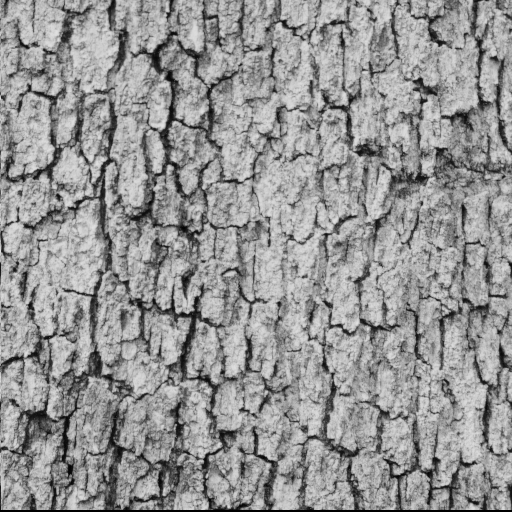
\includegraphics[width=.23\linewidth]{Figures/1102.png}
		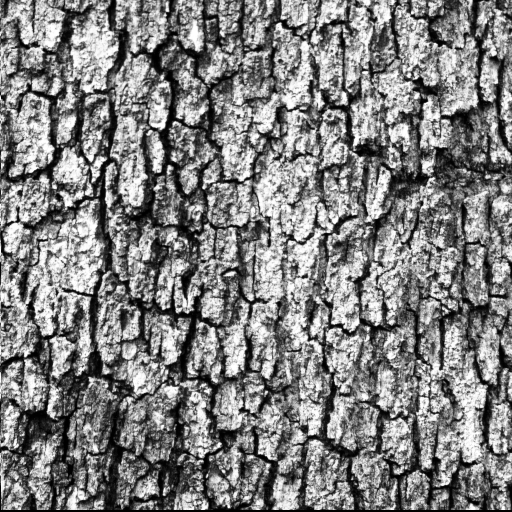
\includegraphics[width=.23\linewidth]{Figures/1202.png}
		\caption{Mesma textura com diferentes contrastes aplicados}
		\label{fig:TwoTexturesDifferentContrast}
	\end{figure}
	
	Sabendo que a curva de \texttt{Hilbert} é aplicada apenas em dados bidimensionais com dimensões em potência de $2$, criamos nossas amostras de dimensão $128 \times 128$ por meio das suas respectivas imagens originais, realizando um corte a partir do ponto $(0,0)$.
	
	Três analises foram realizadas para este estudo onde aplicamos os diferentes métodos de mapeamento relatados anteriormente.
	Nas técnicas de rasterização, cada amostra foi redimensionada para um conjunto de matrizes obtidas de partições deslizantes da imagem onde testamos diversos valores de $D$ para as dimensões $D_{x}$ e $D_{y}$ das partições geradas. 
	O processo de simbolização de Bandt-Pompe foi realizado para cada partição, sendo importante salientar que cada dimensão $D_{x}$ e $D_{y}$ leva a $(D_{x}D_{y})!$ possíveis padrões ordinais. 
	
	Uma das questões de pesquisa consistia em estudar o impacto da equalização dos histogramas de intensidade das texturas nos descritores. 
	Para isto, verificamos o comportamento dos parâmetros da caracterização (dimensão e delay) quando fornecemos como entrada texturas com e sem modificações de contraste. 
	O resultado pode ser observado na figura~\ref{fig:TexturesContrast}, onde podemos perceber que os pontos de mesma cor, ou seja, as diferentes representações de uma textura se sobrepõem, assim como era esperado. 
	Uma vez que a distribuição de Bandt \& Pompe~\cite{Bandt2002Permutation} é resistente a diferentes tipos de contaminação, era esperado que alterações de contraste não alterassem ou apenas provocasse pequenas alterações locais no conjunto total de padrões.
	
	\begin{figure}[!h]
		\centering
		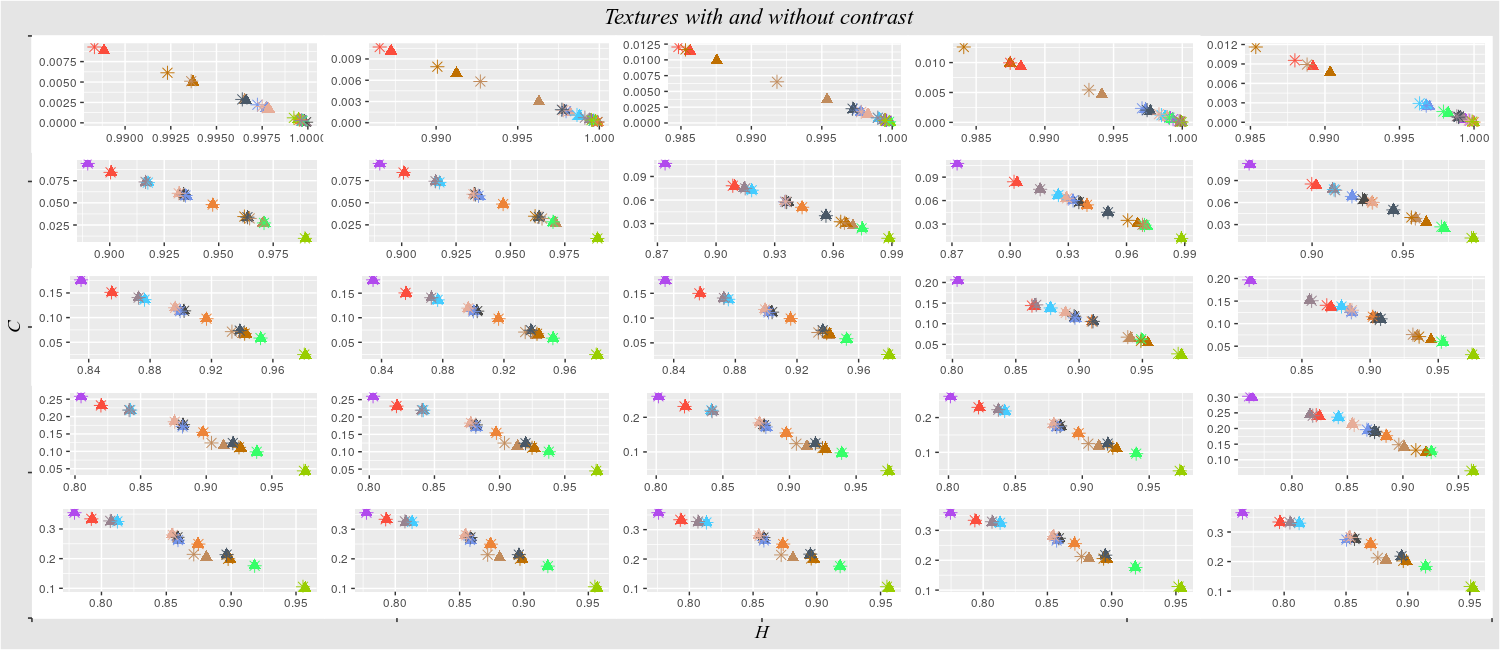
\includegraphics[scale = 0.4]{Figures/TexturesContrast.png}    
		\caption{Caracterização dos dados com e sem modificação do contraste. Os gráficos evoluem horizontalmente de acordo com a dimensão $D$ escolhida e verticalmente com o delay $\tau$}
		\label{fig:TexturesContrast}
	\end{figure}
	
	Como pode ser visto na figura~\ref{fig:AnalysisTextures}, mais uma etapa foi adicionada na análise dos dados provenientes das texturas de Brodatz. 
	Após realizar a caracterização inicial no plano Entropia-Complexidade, verificamos o poder de discriminação destes descritores com o uso do algoritmo DBSCAN~\cite{Ester1996DBSCAN}. 
	
	Sendo um importante método na identificação de padrões ou tendências, os algoritmos de clusterização dividem um conjunto de objetos em subpopulações significativas.
	Particularmente, o algoritmo DBSCAN consiste de uma técnica não-paramétrica que utiliza a densidade de uma vizinhança de objetos para realizar o agrupamento dos dados.
	
	Cada ponto no plano possui valores de entropia e complexidade associados. Logo, a utilização de um método usado para descobrir clusters no espaço será eficaz quando aplicado ao plano. 
	Os pontos agrupados em um cluster devem não ser apenas semelhantes espacialmente, mas também em sua dinâmica.
	
	Dentre as funções de mapeamento analisadas, verificamos que os agrupamentos mais esparços se deram através da curva de \texttt{Hilbert}. Os melhores resultados dentre o total de combinações dos parâmetros de análise podem ser observados na figura~\ref{fig:DBSCAN}.
	
	\begin{figure}[!h]
		\centering
		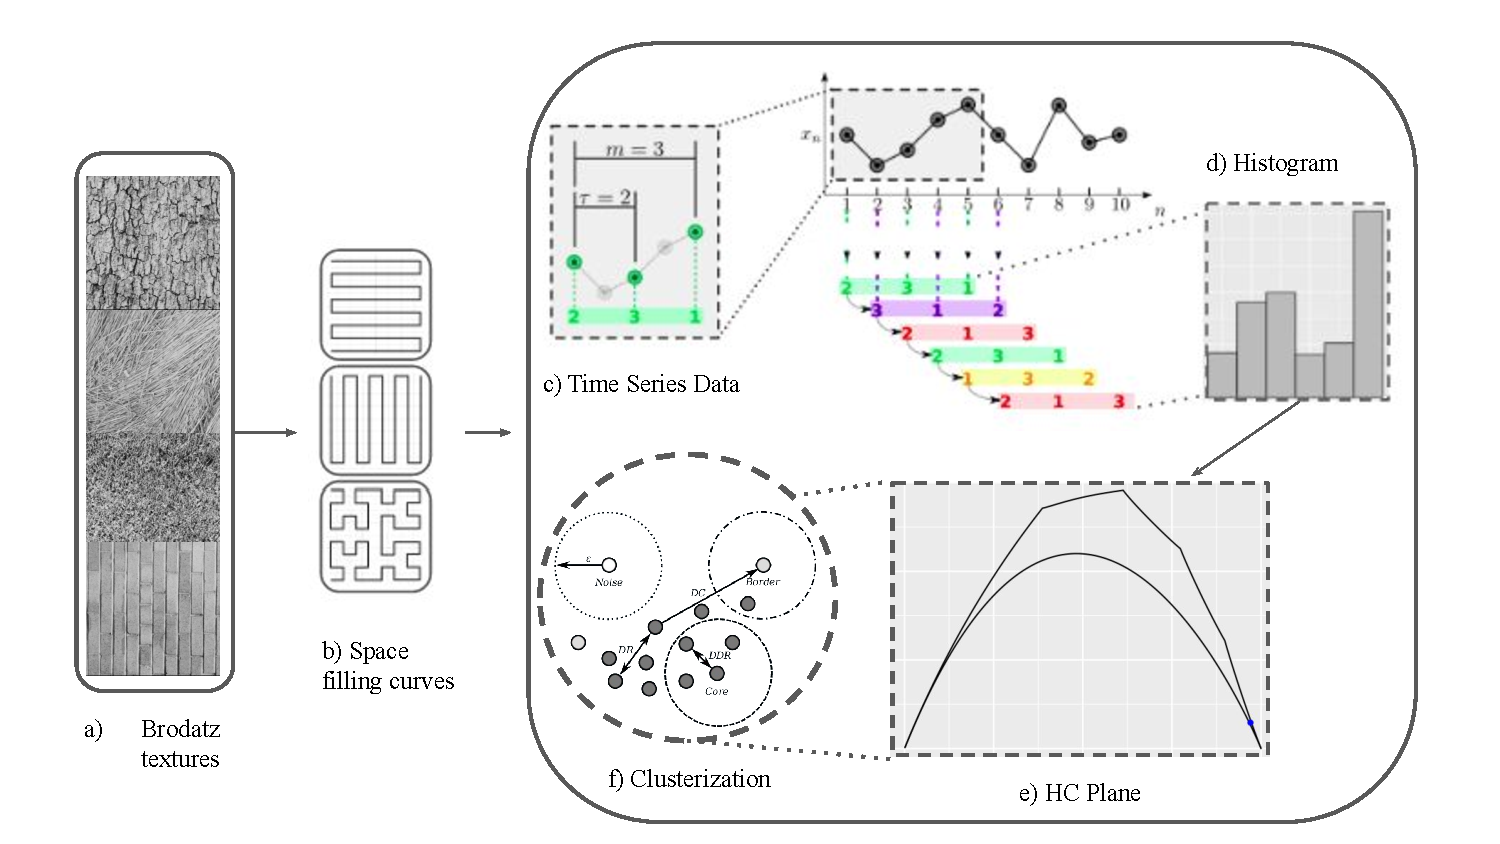
\includegraphics[scale = 0.5]{Figures/AnalysisTextures.pdf}    
		\caption{Etapas da análise realizada na caracterização das texturas de Brodatz}
		\label{fig:AnalysisTextures}
	\end{figure}
	
	\begin{figure}[!h]
		\centering
		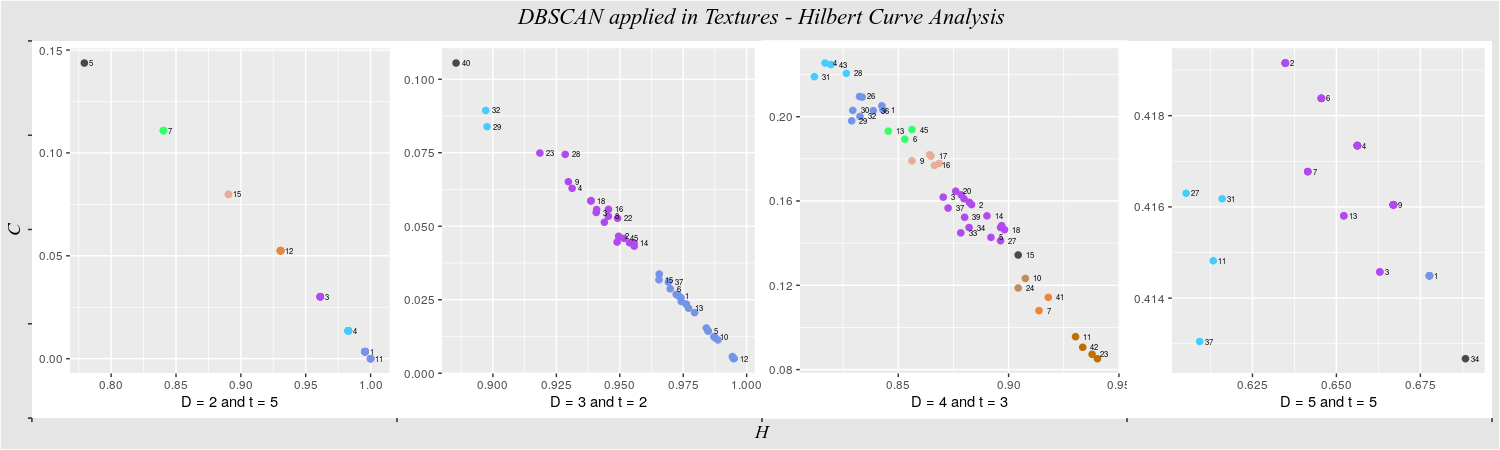
\includegraphics[scale = 0.4]{Figures/DBSCANgrouphilbert.png}    
		\caption{Clusterização aplicada sobre o Plano Entropia-Complexidade}
		\label{fig:DBSCAN}
	\end{figure}
	
	\newpage
	
	\subsection{Imagens SAR}\label{SAR}
	
	Amplamente utilizadas no reconhecimento de características e padrões geográficos, imagens de radar de abertura sintética (\texttt{SAR}) são ricas em informações de textura. Para esta análise, três imagens \texttt{SAR} com diferentes regiões foram usadas, são elas:
	
	\begin{itemize}
		\item Parque Nacional Sierra del Lacandon, Guatemala (adquirido em 10 de abril de 2015), disponível em \url{https://uavsar.jpl.nasa.gov/cgi-bin/product.pl?jobName=Lacand_30202_15043_006_150410_L090_CX_01#dados};
		\item Regiões oceânicas do Cabo Canaveral (adquirido em 22 de setembro de 2016);
		\item Área urbana da cidade de Munique, na Alemanha (adquirido em 5 de junho de 2015).
	\end{itemize}
	
	As imagens usadas neste experimento são resultados da banda HHHH \texttt{SAR} e assim como as amostras das texturas de Brodatz, cada amostra de \texttt{SAR} é representada por uma subimagem de $128 \times 128$.
	
	Um total de 160 amostras foram consideradas durante a investigação, sendo 40 amostras de cada categoria de regiões, são elas: regiões florestais da Guatemala; regiões oceânicas de Cape Canaveral com comportamento 1; regiões oceânicas de Cape Canaveral com comportamento 2 e regiões urbanas da cidade de Munique. Para ilustrar melhor o conjunto de amostras gerado, a figura~\ref{fig:RegioesSAR} exemplifica cada uma das categorias presentes.
	
	\begin{figure}[!h]
		\centering
		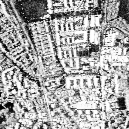
\includegraphics[width=.23\linewidth]{Figures/munichUrban.png}
		
\includegraphics[width=.23\linewidth]{Figures/Cape1.png}
		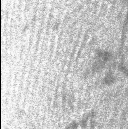
\includegraphics[width=.23\linewidth]{Figures/Cape2.png}
		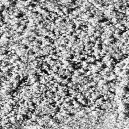
\includegraphics[width=.23\linewidth]{Figures/guatemalaflorest.png}
		\caption{Tipos de regiões analisadas: (a) Regiões urbanas; (b) Região Oceânica Tipo 1; (c) Região Oceânica Tipo 2 e (d) Regiões Florestais.}\label{fig:RegioesSAR}
	\end{figure}
	
	Novamente foram feitas três análises seguindo a metodologia proposta. Como pode ser observado na figura~\ref{fig:sinaisSAR}, embora apresentem formas semelhantes de varredura, podemos verificar que existe uma discrepância nos sinais gerados pelas curvas de rasterização. 
	
	Neste trabalho, demos mais atenção ao resultado da caracterização obtida por meio da curva de \texttt{Hilbert}.
	Na figura~\ref{Fig:PlotsHilbert} podemos visualizar o resultado da caracterização das diferentes regiões analisadas e notar algumas considerações:
	
	\begin{enumerate}
		\item Os pontos de regiões de Cape Canaveral com comportamento diferentes se misturam em grande parte dos gráficos. Este comportamento se assemelha ao teste de impacto da equalização dos histogramas de intensidade realizado no exemplo anterior. Como ilustrado na figura~\ref{fig:RegioesSAR}, as texturas possuem características visuais semelhantes, sendo esperado que seus valores de entropia e complexidade também se assemelhem.
		\item Com o aumento do parâmetro $\tau$ verificamos que os pontos das áreas florestais da Guatemala ficam mais dispersos, com uma complexidade estatística maior e consequentemente com uma menor entropia. Quando observamos $\tau = 1$, a entropia das amostras estão próximas do valor máximo, indicando que se tratam de texturas pouco uniformes e com um alto grau de incoerência, assim como observado na figura~\ref{fig:RegioesSAR}.
		\item A caracterização das amostras de áreas urbanas de Munique nos mostra que quanto maior o parâmetro $D$ menor a entropia e maior a complexidade estatística dos respectivos sinais unidimensionais. Tal fato se deve ao aumento de informação fornecida pelos sinais. Uma vez que estamos analisando regiões urbanas, quanto maior a área de interesse da análise maior a ocorrência de padrões e estruturas na dinâmica dos sinais verificados.
	\end{enumerate}
	
	\begin{figure}[!h]
		\centering
		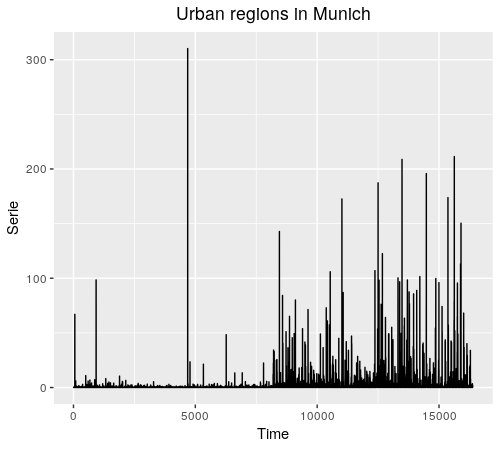
\includegraphics[width=.3\linewidth]{Figures/munichhilbert.png}
		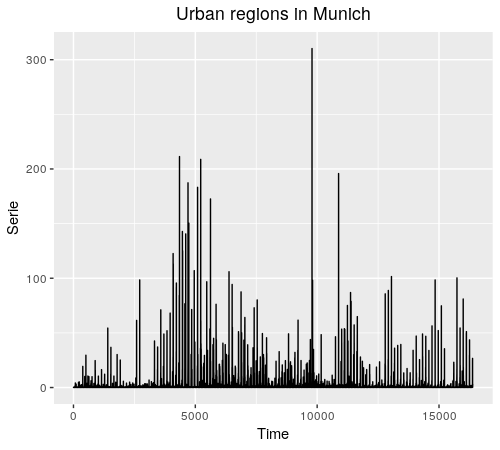
\includegraphics[width=.3\linewidth]{Figures/munichraster1.png}
		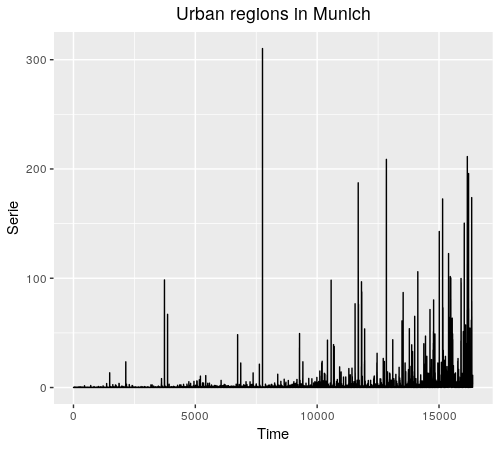
\includegraphics[width=.3\linewidth]{Figures/munichraster2.png}
		\caption{Análise dos sinais de uma amostra de região urbana de Munique seguindo as três curvas de varredura: (a) Curva de \texttt{Hilbert}; (b) \texttt{Raster-1} e (c) \texttt{Raster-2}}\label{fig:sinaisSAR}
	\end{figure}
	
	
	\begin{figure}[!h]
		\begin{tabular}{c}
			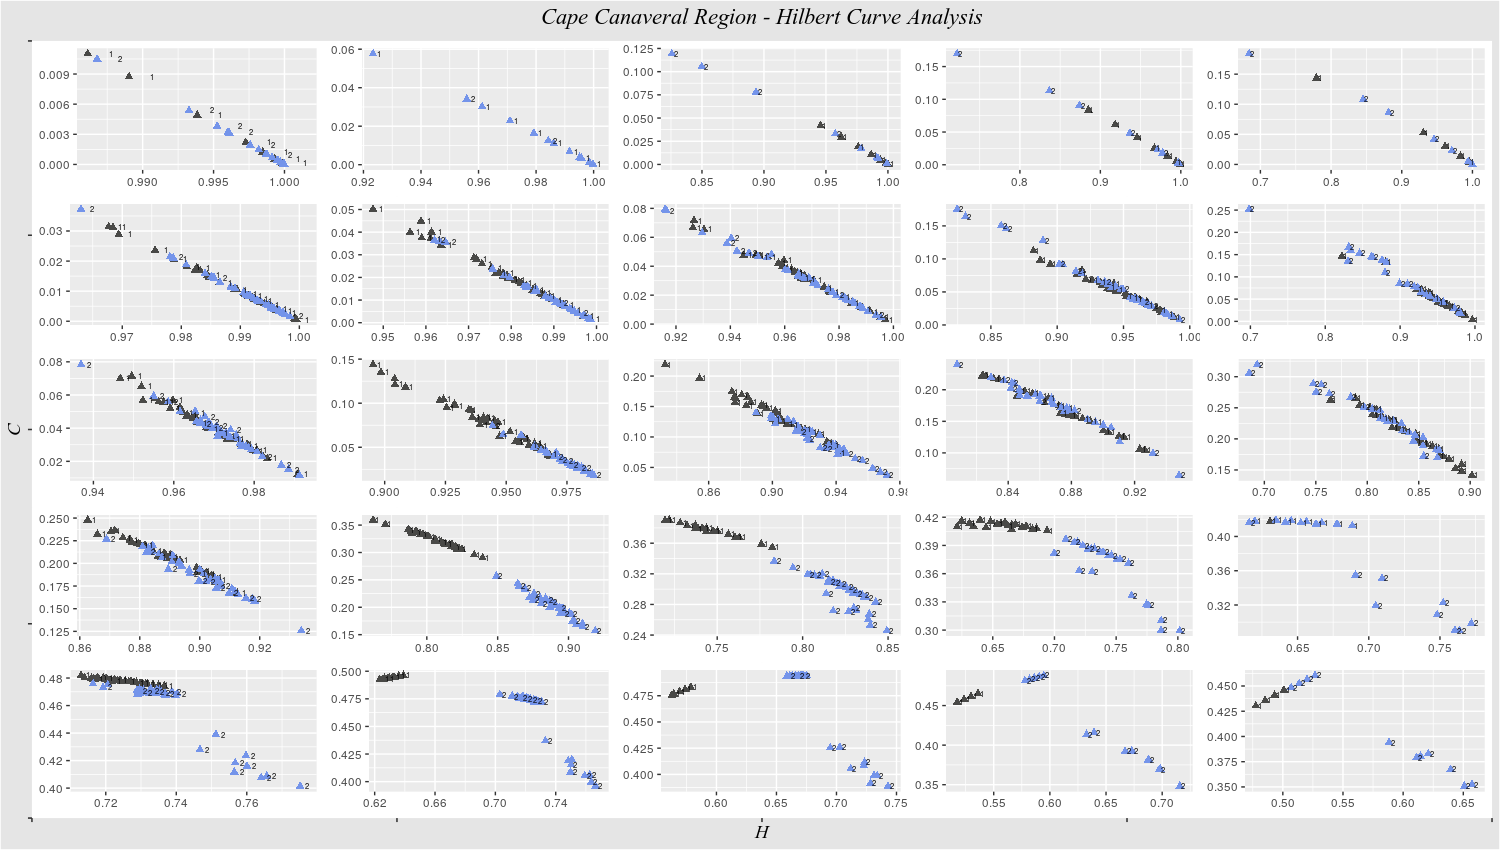
\includegraphics[width=0.9\textwidth]{Figures/CapehilbertPlots.png}\\
			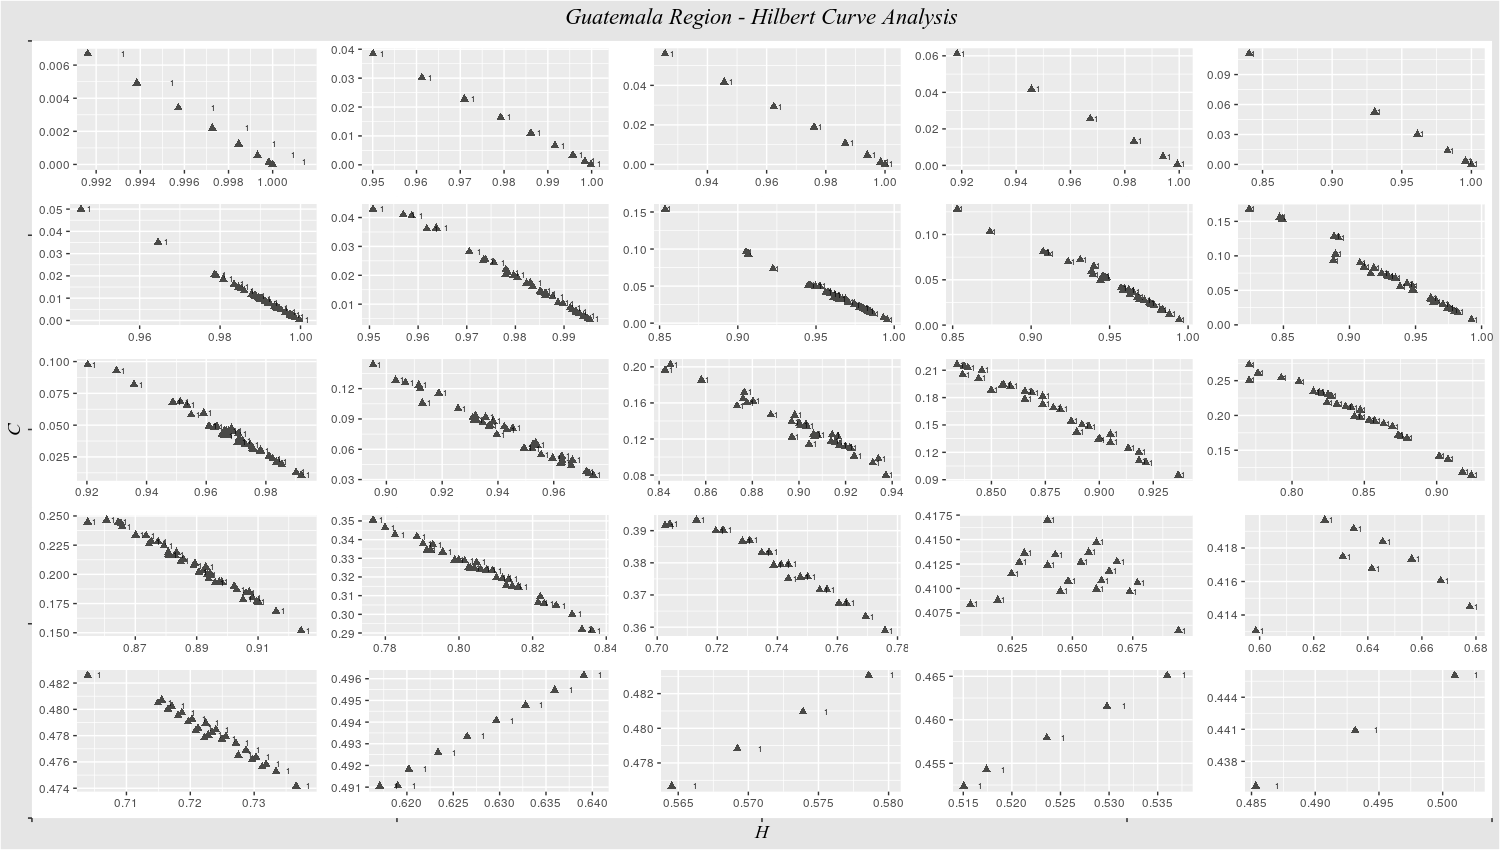
\includegraphics[width=0.9\textwidth]{Figures/GuatemalahilbertPlots.png}\\
			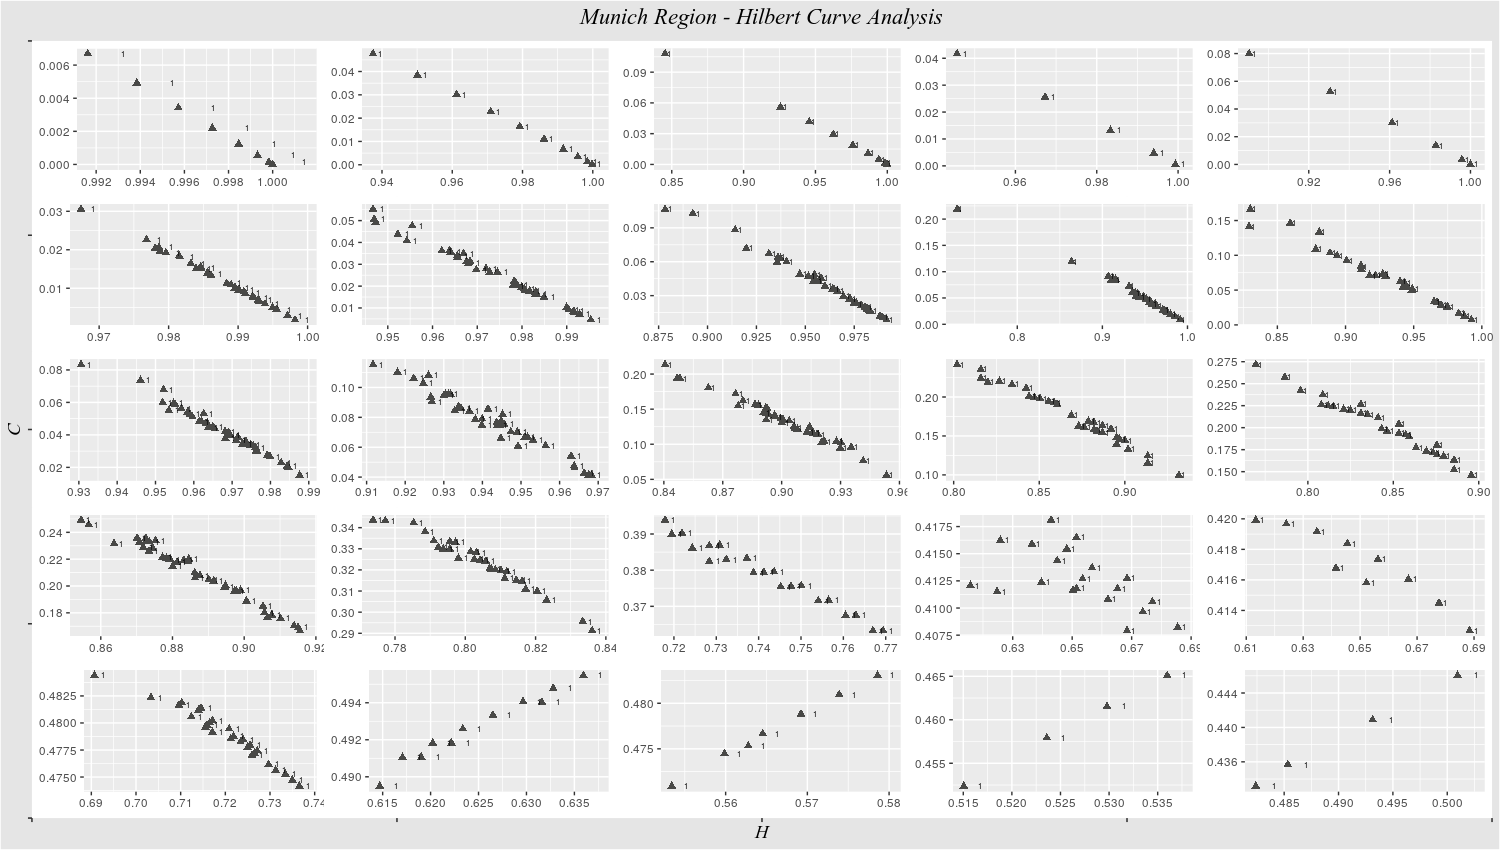
\includegraphics[width=0.9\textwidth]{Figures/MunichhilbertPlots.png}\\
		\end{tabular}
		\caption{Caracterização resultante da aplicação da curva de \texttt{Hilbert} sobre texturas de diferentes regiões: (a) Cape de Canaveral (pontos azul representam o comportamento 1 e pontos cinza o comportamento 2); (b) Guatemala e (c) Munique.}
		\label{Fig:PlotsHilbert}
	\end{figure}
	
	%%%%%%%%%%%%%%%%%%%%%%%%%%%%%%%%%%%%%%%%%%
	\section{Conclusões e trabalhos futuros}\label{conclusao}
	
	A partir dos resultados apresentados, podemos concluir que, para os exemplos tratados, a utilização de \textit{space filling curves} aliadas à descritores da Teoria da Informação mostram possuir um desempenho discriminativo promissor para análise de texturas, em especial para texturas provenientes de imagens \texttt{SAR}, onde o poder da caracterização pode se tornar uma eficiente ferramenta de análise da semântica de diferentes regiões.
	
	Deve-se notar que o presente estudo consiste em uma avaliação preliminar das características propostas, realizada apenas com três imagens \texttt{SAR}. Pesquisas e análises adicionais estão em andamento para avaliar o desempenho discriminante de tais descritores. Além disso, em trabalhos futuros serão levados em consideração a adição de mais um novo parâmetro na caracterização: o parâmetro Alpha. Baseline com técnicas propostas na literatura também será implementado para validar a nossa metodologia.
	
	%%%%%%%%%%%%%%%%%%%%%%%%%%%%%%%%%%%%%%%%%%
	%section{Patents}
	%This section is not mandatory, but may be added if there are patents resulting from the work reported in this manuscript.
	
	%%%%%%%%%%%%%%%%%%%%%%%%%%%%%%%%%%%%%%%%%%
	\vspace{6pt} 
	
	%%%%%%%%%%%%%%%%%%%%%%%%%%%%%%%%%%%%%%%%%%
	%% optional
	%\supplementary{The following are available online at \linksupplementary{s1}, Figure S1: title, Table S1: title, Video S1: title.}
	
	% Only for the journal Methods and Protocols:
	% If you wish to submit a video article, please do so with any other supplementary material.
	% \supplementary{The following are available at \linksupplementary{s1}, Figure S1: title, Table S1: title, Video S1: title. A supporting video article is available at doi: link.}
	
	%%%%%%%%%%%%%%%%%%%%%%%%%%%%%%%%%%%%%%%%%%
	%\authorcontributions{For research articles with several authors, a short paragraph specifying their individual contributions must be provided. The following statements should be used “conceptualization, X.X. and Y.Y.; methodology, X.X.; software, X.X.; validation, X.X., Y.Y. and Z.Z.; formal analysis, X.X.; investigation, X.X.; resources, X.X.; data curation, X.X.; writing—original draft preparation, X.X.; writing—review and editing, X.X.; visualization, X.X.; supervision, X.X.; project administration, X.X.; funding acquisition, Y.Y.”, please turn to the  \href{http://img.mdpi.org/data/contributor-role-instruction.pdf}{CRediT taxonomy} for the term explanation. Authorship must be limited to those who have contributed substantially to the work reported.}
	
	%%%%%%%%%%%%%%%%%%%%%%%%%%%%%%%%%%%%%%%%%%
	%\funding{Please add: ``This research received no external funding'' or ``This research was funded by NAME OF FUNDER grant number XXX.'' and  and ``The APC was funded by XXX''. Check carefully that the details given are accurate and use the standard spelling of funding agency names at \url{https://search.crossref.org/funding}, any errors may affect your future funding.}
	
	%%%%%%%%%%%%%%%%%%%%%%%%%%%%%%%%%%%%%%%%%%
	%\acknowledgments{In this section you can acknowledge any support given which is not covered by the author contribution or funding sections. This may include administrative and technical support, or donations in kind (e.g., materials used for experiments).}
	
	%%%%%%%%%%%%%%%%%%%%%%%%%%%%%%%%%%%%%%%%%%
	%\conflictsofinterest{The authors declare no conflict of interest.} 
	
	%%%%%%%%%%%%%%%%%%%%%%%%%%%%%%%%%%%%%%%%%%
	%% optional
	%\abbreviations{The following abbreviations are used in this manuscript:\\
	
	%\noindent 
	%\begin{tabular}{@{}ll}
	%MDPI & Multidisciplinary Digital Publishing Institute\\
	%DOAJ & Directory of open access journals\\
	%TLA & Three letter acronym\\
	%LD & linear dichroism
	%\end{tabular}}
	
	%%%%%%%%%%%%%%%%%%%%%%%%%%%%%%%%%%%%%%%%%%
	%% optional
	%\appendixtitles{no} %Leave argument "no" if all appendix headings stay EMPTY (then no dot is printed after "Appendix A"). If the appendix sections contain a heading then change the argument to "yes".
	%\appendixsections{multiple} %Leave argument "multiple" if there are multiple sections. Then a counter is printed ("Appendix A"). If there is only one appendix section then change the argument to "one" and no counter is printed ("Appendix").
	%\appendix
	%\section{}
	%\unskip
	%The appendix is an optional section that can contain details and data supplemental to the main text. For example, explanations of experimental details that would disrupt the flow of the main text, but nonetheless remain crucial to understanding and reproducing the research shown; figures of replicates for experiments of which representative data is shown in the main text can be added here if brief, or as Supplementary data. Mathematical proofs of results not central to the paper can be added as an appendix. 
	
	%%%%%%%%%%%%%%%%%%%%%%%%%%%%%%%%%%%%%%%%%%
	% Citations and References in Supplementary files are permitted provided that they also appear in the reference list here. 
	
	%=====================================
	% References, variant A: internal bibliography
	%=====================================
	\reftitle{References}
	%\begin{thebibliography}{999}
	% Reference 1
	%\bibitem[Author1(year)]{ref-journal} 
	%Author1, T. The title of the cited article. {\em Journal Abbreviation} {\bf 2008}, {\em 10}, 142-149, doi:xxxxx.
	% Reference 2
	%\bibitem[Author2(year)]{ref-book} 
	%Author2, L. The title of the cited contribution. In {\em The Book Title}; Editor1, F., Editor2, A., Eds.; Publishing House: City, Country, 2007; pp. 32-58, ISBN.
	%\end{thebibliography}
	
	% The following MDPI journals use author-date citation: Arts, Econometrics, Economies, Genealogy, Humanities, IJFS, JRFM, Laws, Religions, Risks, Social Sciences. For those journals, please follow the formatting guidelines on http://www.mdpi.com/authors/references
	% To cite two works by the same author: \citeauthor{ref-journal-1a} (\citeyear{ref-journal-1a}, \citeyear{ref-journal-1b}). This produces: Whittaker (1967, 1975)
	% To cite two works by the same author with specific pages: \citeauthor{ref-journal-3a} (\citeyear{ref-journal-3a}, p. 328; \citeyear{ref-journal-3b}, p.475). This produces: Wong (1999, p. 328; 2000, p. 475)
	
	%=====================================
	% References, variant B: external bibliography
	%=====================================
	\externalbibliography{yes}
	\bibliography{../../Common/references}
	
	%%%%%%%%%%%%%%%%%%%%%%%%%%%%%%%%%%%%%%%%%%
	%% optional
	%\sampleavailability{Samples of the compounds ...... are available from the authors.}
	
	%% for journal Sci
	%\reviewreports{\\
	%Reviewer 1 comments and authors’ response\\
	%Reviewer 2 comments and authors’ response\\
	%Reviewer 3 comments and authors’ response
	%}
	
	%%%%%%%%%%%%%%%%%%%%%%%%%%%%%%%%%%%%%%%%%%
\end{document}

